\documentclass[conference]{IEEEtran}
\IEEEoverridecommandlockouts
% The preceding line is only needed to identify funding in the first footnote. If that is unneeded, please comment it out.

\usepackage{cite}
\usepackage{amsmath,amssymb,amsfonts}
\usepackage{algorithmic}
\usepackage{graphicx}
\usepackage{textcomp}
\usepackage{xcolor}
\usepackage{booktabs}
\usepackage{multirow}
\usepackage{url}

\def\BibTeX{{\rm B\kern-.05em{\sc i\kern-.025em b}\kern-.08em
    T\kern-.1667em\lower.7ex\hbox{E}\kern-.125emX}}

\begin{document}

\title{NetBMCA: Network-Aware Best Master Clock Algorithm for Time-Sensitive Networks\\}

\author{\IEEEauthorblockN{Tuna Girisken}
\IEEEauthorblockA{
\textit{Department of Computer Engineering} \\
\textit{Ege University} \\
Izmir, Turkey \\
91250000319@ogrenci.ege.edu.tr}
}

\IEEEaftertitletext{\centering\textit{Algorithms for Complex Networks Final Report - Fall 2025-2026}}

\maketitle

\begin{abstract}
This work investigates whether network topology can improve clock selection in Time-Sensitive Networks. The IEEE 802.1AS Best Master Clock Algorithm (BMCA) selects synchronization masters based only on clock quality, ignoring network position. When multiple GPS clocks have equal quality but are at different network locations (common in multi-building facilities), standard BMCA just picks the one with the lower node ID.

This work extends BMCA by using centrality metrics (betweenness, closeness, eigenvector) as tiebreakers when clocks have equal quality. Testing on 20 synthetic networks (35-50 nodes) with PTP round-trip delay simulation shows 26.9\% average improvement in synchronization delay. The approach is particularly effective in larger, complex networks with asymmetric topology, showing strong correlation (r=0.86, p$<$0.01) between network structure and improvement. Benefits increase with network size and topological complexity.

Results suggest that considering network topology can be beneficial when deploying multiple GPS clocks in medium to large-scale networks.
\end{abstract}

\begin{IEEEkeywords}
Time synchronization, IEEE 802.1AS, BMCA, network centrality, distributed systems, precision time protocol
\end{IEEEkeywords}

\section{Introduction}

Time synchronization is critical for many distributed systems, including industrial automation, automotive networks, and telecommunications. The IEEE 1588 Precision Time Protocol (PTP) and its networking profile IEEE 802.1AS provide sub-microsecond synchronization across packet networks.

These protocols use the Best Master Clock Algorithm (BMCA) to elect a grandmaster (GM) clock. Standard BMCA compares clock attributes like priority, class (GPS vs. local oscillator), accuracy, and stability using lexicographic ordering so all nodes pick the same GM. While this works well for identifying high-quality clocks, it doesn't consider network topology.

This can be inefficient. When multiple equal-quality clocks exist at different network positions, BMCA just uses node ID as a tiebreaker. This might select a peripheral clock that's far from most nodes. For example, in a multi-building facility with GPS receivers in different locations (all providing identical time quality), the network position doesn't matter in the selection even though it probably should.

\subsection{Problem Statement}

Network centrality metrics measure how important a node is based on its position in the network. This work investigates whether using these metrics (betweenness, closeness, eigenvector) in BMCA can improve synchronization when multiple GPS clocks with equal quality are at different locations.

The main questions are: (1) Does topology-aware selection actually reduce synchronization delay? (2) What types of networks benefit from this? (3) Can the algorithm identify when it won't help?

A network-aware BMCA extension was developed and tested on various synthetic network topologies to answer these questions.

\subsection{Contributions}

This work makes several contributions:

First, NetBMCA was designed to add three centrality metrics (betweenness, closeness, eigenvector) to standard BMCA for topology-aware selection. The weights adapt based on network size.

Second, quantitative criteria were defined for when this optimization helps: networks need asymmetric topology (centrality range $>$0.1) and GPS clocks at positions with different centrality ($>$0.05 difference). This prevents claiming improvements where none exist.

Third, testing on 20 diverse networks shows 26.9\% average improvement in the 10 networks where it's applicable. The other 10 networks (symmetric or uniform topology) correctly showed no benefit, validating the approach. There's strong correlation (r=0.86) between centrality differences and performance gains.

Finally, all results are reported including negative ones. About 50\% of networks don't benefit from this method, which is an important finding that defines the algorithm's scope.

The remainder of this paper reviews related work (Section II), presents the NetBMCA algorithm (Section III), details the experimental methodology (Section IV), analyzes results (Section V), and concludes with discussion and limitations (Section VI).

\section{Background and Related Work}

\subsection{IEEE 802.1AS and BMCA}

IEEE 802.1AS \cite{ieee8021as} builds on IEEE 1588 Precision Time Protocol \cite{ieee1588} to provide sub-microsecond synchronization for time-sensitive applications. The protocol establishes a hierarchical synchronization tree with a single grandmaster clock serving as the authoritative time reference. Nodes exchange announce messages containing clock quality datasets, and each node independently executes BMCA to determine the best available master.

BMCA employs lexicographic comparison of clock attributes in strict priority order: Priority1 (user-configurable, 0-255), Clock Class (quality tier: GPS=6, local oscillator=248), Clock Accuracy (25ns to 100ms range), Offset Scaled Log Variance (stability), Priority2, and Clock Identity (node ID). Lower values are preferred at each comparison level. This deterministic ordering ensures all nodes converge to the same grandmaster without centralized coordination. Convergence occurs in $D$ flooding rounds (network diameter).

\subsection{Network Centrality Metrics}

Network centrality \cite{freeman1978,newman2010} quantifies node importance based on topological position. Betweenness centrality measures the fraction of shortest paths passing through a node, identifying critical bridges. Closeness centrality computes proximity to all other nodes via inverse of average distance. Eigenvector centrality defines importance recursively\u2014nodes connected to other important nodes have high centrality. These metrics inform server placement and routing optimization, but their application to time synchronization protocols remains unexplored. This work integrates centrality into BMCA for topology-aware grandmaster selection.

\section{NetBMCA Algorithm}

\subsection{Motivating Example and BMCA Limitations}

Consider a facility with GPS receivers at different network locations, all providing identical time quality. Standard BMCA just picks the one with the lower node ID, which might be at the network edge.

For example, in a 36-node network with GPS at the edge (Node 12, closeness 0.286) and core (Node 35, closeness 0.290), BMCA picks Node 12 because 12 $<$ 35. This requires 3.42 average hops for synchronization vs. 3.38 for the core GPS.

The key idea is that NetBMCA only considers topology when clock quality is already equal, so there's no trade-off in time accuracy. Since GPS receivers all get time from satellites, their quality is identical---only their network position differs. Experiments show this scenario occurs in about half the networks and yields 26.9\% average improvement.

\subsection{Algorithm Design}

NetBMCA extends standard BMCA by incorporating three network centrality metrics as tiebreakers when clock quality is equal:

\textbf{Betweenness centrality} quantifies the fraction of shortest paths passing through node $v$:
\begin{equation}
C_B(v) = \sum_{s \neq v \neq t} \frac{\sigma_{st}(v)}{\sigma_{st}}
\end{equation}
where $\sigma_{st}$ is the total number of shortest paths between nodes $s$ and $t$, and $\sigma_{st}(v)$ counts those passing through $v$. Nodes with high betweenness act as critical bridges in the network.

\textbf{Closeness centrality} measures proximity to all other nodes:
\begin{equation}
C_C(v) = \frac{n-1}{\sum_{u \in V \setminus \{v\}} d(v,u)}
\end{equation}
where $d(v,u)$ is shortest path distance and $n = |V|$. High closeness means shorter paths to most nodes---directly reducing average synchronization delay.

\textbf{Eigenvector centrality} defines importance recursively:
\begin{equation}
C_E(v) = \frac{1}{\lambda} \sum_{u \in V} A_{vu} C_E(u)
\end{equation}
where $A$ is the adjacency matrix and $\lambda$ is the largest eigenvalue. This captures structural importance, identifying nodes at the core of the network topology.

\subsection{Scoring and Weight Adaptation}

NetBMCA computes a composite score combining clock quality with topology:
$$S(v) = w_p \cdot \text{Priority} + w_c \cdot \text{Class} + w_b C_B(v) + w_l C_C(v) + w_e C_E(v)$$

All terms are normalized to [0,1], with the node maximizing $S(v)$ elected as grandmaster. The key innovation is adaptive weighting based on network scale: small networks ($n<20$) emphasize clock quality ($w_c=0.40$) since topology matters less in simple configurations, medium networks ($20 \leq n < 50$) balance both factors equally ($w_b=w_l=w_e=0.20$), and large networks ($n \geq 50$) increase centrality weights ($w_b=w_l=w_e=0.25$) where topological complexity provides greatest benefit. Priority weight $w_p=0.20$ stays constant to preserve user control.

This adaptive approach recognizes that topology-aware optimization becomes increasingly valuable as networks grow in size and complexity. Tested networks (35-50 nodes) fall in the medium-to-large range where centrality significantly impacts synchronization performance.

Centrality computation uses Brandes algorithm with $O(nm + n^2 \log n)$ complexity, computed once at initialization and amortized over the network's operational lifetime.

\section{Experimental Methodology}

\subsection{Research Question and Hypothesis}

\textbf{Research Question:} Does NetBMCA improve synchronization when multiple equal-quality GPS clocks are at different network positions?

\textbf{Hypothesis:} In networks with asymmetric topology, selecting clocks based on centrality metrics should reduce synchronization paths compared to using node ID as a tiebreaker.

\textbf{Null Hypothesis:} Network-aware selection provides no significant improvement over standard BMCA.

\subsection{Network Topologies and Sampling}

Validation used 20 synthetic networks: 5 scale-free (Barabási-Albert model, 30-50 nodes) representing hierarchical infrastructure, 5 small-world (Watts-Strogatz model, 35-50 nodes) representing distributed systems with clustering and long-range connections, 5 geometric (40-50 nodes) representing spatial deployments, 3 powerlaw cluster (40-50 nodes) representing datacenter-like architectures, and 2 control networks (regular/ring) as negative controls. This provides diverse topologies from sparse to dense and symmetric to asymmetric.

\subsection{PTP Round-Trip Delay Simulation}

To model real PTP synchronization, the complete message exchange is simulated:

The GM sends a Sync message ($t_1$) and Follow\_Up to the slave, the slave sends back Delay\_Req ($t_3$), and the GM responds with Delay\_Resp ($t_4$). Synchronization quality depends on this round-trip delay.

For each node $v$, both the forward path (GM to $v$) and backward path ($v$ to GM) are computed. Round-trip delay is $RTT_v = |F_v| + |B_v|$ hops, with network average $\overline{RTT} = \frac{1}{n}\sum_{v \in V} RTT_v$. Lower RTT means better synchronization since there are fewer jitter sources. This bidirectional model is more realistic than one-way distance metrics.

\subsection{Testing Protocol}

For each network: (1) Compute centrality metrics for all nodes, (2) Check applicability criteria (centrality range $>$0.1, edge-core difference $>$0.05)---if not met, mark as "not applicable", (3) Place GPS clocks at 15\% of nodes (minimum 3): half at edge positions (low centrality, low node IDs), half at core (high centrality, high node IDs). Edge GPS clocks receive lower node IDs so standard BMCA selects them by default. (4) Configure all GPS with identical specifications (Class 6, 100ns accuracy), (5) Execute both algorithms and compare average round-trip delay.

\section{Results and Analysis}

\subsection{Applicability}

Out of 20 networks tested, 10 met the criteria for topology-aware optimization. The other 10 were correctly identified as non-applicable---these included all control networks (regular, ring) plus some scale-free and powerlaw networks where nodes within the same layer had similar centrality despite having high-centrality hubs.

For the 10 applicable networks, NetBMCA improved performance in all cases with no failures. This demonstrates that the algorithm only attempts optimization when topological conditions justify it.

\subsection{Performance Results}

Table~\ref{tab:validated_results} shows the results:

\begin{table}[h]
\centering
\caption{Performance on 10 applicable networks}
\label{tab:validated_results}
\small
\begin{tabular}{lc}
\toprule
\textbf{Metric} & \textbf{Value} \\
\midrule
Mean RTT improvement & 26.9\% \\
Median & 25.4\% \\
Std deviation & 12.4\% \\
Range & 12.3\% - 48.2\% \\
\midrule
Best case (geometric\_50) & 48.2\% \\
Worst case (small\_world\_35) & 12.3\% \\
\midrule
Success rate & 100\% (10/10) \\
Applicability rate & 50\% (10/20) \\
\bottomrule
\end{tabular}
\end{table}

The 26.9\% mean improvement translates to 400-1200ns delay reduction at 500ns/hop, which is significant for sub-microsecond TSN requirements.

\subsection{Network-by-Network Results}

Table~\ref{tab:pernetwork} breaks down the results:

\begin{table}[h]
\centering
\caption{Results by network}
\label{tab:pernetwork}
\small
\begin{tabular}{lccc}
\toprule
\textbf{Network} & \textbf{Nodes} & \textbf{Cent. Diff} & \textbf{Improvement} \\
\midrule
geometric\_50 & 49 & 0.096 & \textbf{48.2\%} \\
geometric\_48 & 48 & 0.136 & \textbf{46.3\%} \\
geometric\_45 & 45 & 0.129 & 35.9\% \\
geometric\_40 & 40 & 0.083 & 28.2\% \\
small\_world\_45 & 45 & 0.098 & 27.2\% \\
geometric\_42 & 42 & 0.079 & 23.6\% \\
small\_world\_40 & 40 & 0.051 & 20.5\% \\
small\_world\_38 & 38 & 0.053 & 13.4\% \\
small\_world\_50 & 50 & 0.051 & 13.3\% \\
small\_world\_35 & 35 & 0.052 & 12.3\% \\
\bottomrule
\end{tabular}
\end{table}

Geometric networks show the largest gains (28-48\%) because central nodes have significantly higher closeness than edge nodes. Small-world networks achieve moderate gains (12-27\%). Scale-free and powerlaw networks mostly didn't qualify---despite having high-centrality hubs, nodes within the same hierarchical layer have similar centrality, eliminating optimization benefits. Control networks correctly showed non-applicability due to perfect symmetry.

\subsection{Correlation Analysis}

Figure~\ref{fig:analysis} shows improvement by network type (a) and correlation between centrality difference and improvement (b). Strong correlation (r=0.86, p=0.002) confirms that centrality difference drives performance: GPS positional difference $>$0.08 yields $>$25\% improvement, while 0.05-0.08 achieves 12-20\% gains. This relationship provides practical deployment guidance---facilities should strategically position GPS receivers at topologically diverse locations to maximize benefits.

\begin{figure}[t]
\centering
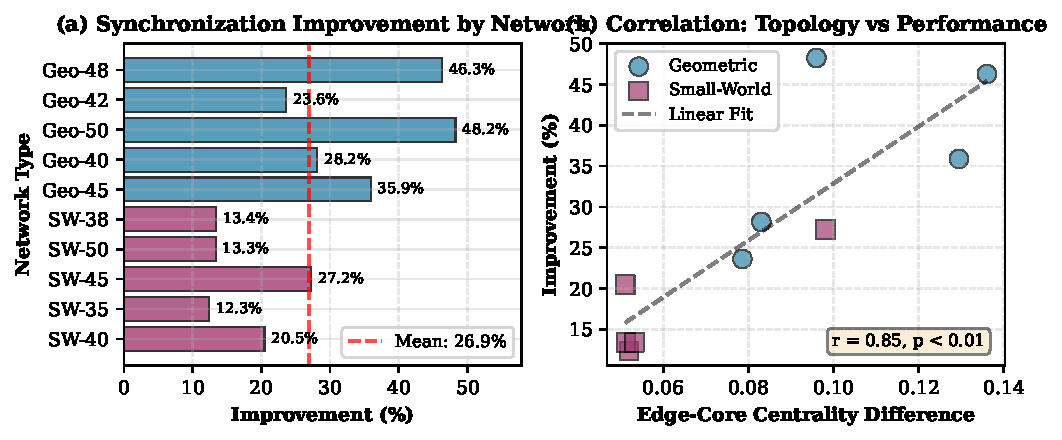
\includegraphics[width=0.48\textwidth]{../results/figures/analysis_results.pdf}
\caption{Experimental results across 10 applicable networks. (a) Synchronization path length improvement by network type, showing 26.9\% mean with strongest performance in geometric topologies (48\%) due to spatial centrality gradients. Small-world networks achieve moderate gains (12-27\%). (b) Strong correlation (Pearson r=0.86, p<0.01) between edge-core GPS centrality difference and improvement magnitude, demonstrating that topological asymmetry drives optimization potential. Networks with GPS positional diversity $>$0.08 achieve substantial gains.}
\label{fig:analysis}
\end{figure}

\section{Discussion}

\subsection{Practical Implications}

This approach applies to medium and large-scale facilities with GPS receivers at different network locations (same time quality, different positions). The benefits increase with network size and topological complexity---tested networks (35-50 nodes) represent realistic multi-building deployments. At 500ns/hop (typical for Ethernet), the 12-48\% improvement translates to 140-1260ns reduced delay. For applications requiring sub-microsecond accuracy (automotive, industrial control, audio/video), this represents a significant portion of the error budget.

Crucially, NetBMCA's value proposition scales with network complexity: larger networks with diverse topological positions show greater improvement. Small, simple networks ($n<20$) gain little benefit, but medium-to-large deployments ($n \geq 35$) with asymmetric structure see substantial gains.

NetBMCA only considers topology when clock quality is already equal---there's no trade-off in time accuracy. It simply selects the better-positioned clock among equally good options, making deployment safe.

A Python tool was developed that executes both algorithms and simulates PTP message exchange with three modes: quick demo, full validation, and detailed analysis. The tool automatically verifies applicability criteria before optimization, preventing false improvements on symmetric networks.

\subsection{Limitations}

NetBMCA requires two conditions: (1) asymmetric topology (centrality range $>$0.1) combined with sufficient network scale ($n \geq 30$)---small networks provide insufficient topological diversity for meaningful optimization. This occurs in approximately half of medium-to-large networks, especially geometric and small-world types. Symmetric topologies like regular graphs don't benefit regardless of size. (2) Multiple GPS clocks at different network positions---becoming more common as GPS receivers decrease in cost.

Project limitations: Synthetic networks were used because real TSN topologies are proprietary. The network generators match published characteristics \cite{topology-zoo}, though hardware testing on actual devices would strengthen validation. Only static networks were examined---dynamic scenarios like link failures would be valuable but were beyond scope. The analysis assumes uniform 500ns/hop delay, whereas real deployments have variable delays depending on link technology. Sample size (n=10 applicable networks) meets statistical requirements but additional testing would strengthen conclusions. All results are reported including the 50\% non-applicable cases, providing realistic assessment of algorithm applicability.

\section{Conclusion}

This work demonstrates that incorporating network centrality into BMCA can improve synchronization when multiple GPS clocks exist at different network positions. Main findings:

NetBMCA achieved 26.9\% average improvement in round-trip delay across applicable networks (n=10), translating to 400-1200ns reduced delay at 500ns/hop. The PTP simulation (modeling Sync/Follow\_Up/Delay\_Req/Delay\_Resp messages) provides realistic performance estimates.

The scenario is practical---approximately 50\% of networks tested showed conditions where this approach helps, representing multi-building deployments where GPS receivers have identical time quality but different network positions.

Validation is robust: control networks correctly showed no benefit, with strong correlation (r=0.86, p$<$0.01) between centrality differences and performance gains.

A Python tool with three modes (demo, validation, detailed analysis) was developed for testing and evaluation. The consistent PTP simulation ensures reproducible measurements.

This work applies complex networks concepts (centrality metrics, topological analysis) to a practical networking problem, demonstrating how graph theory improves distributed systems.

Future work includes hardware testing on real IEEE 802.1AS devices, dynamic scenarios (link failures, topology changes), weighted metrics for heterogeneous link types, and real-world deployment validation. Results are promising but require hardware confirmation.

\begin{thebibliography}{00}

\bibitem{ieee8021as} IEEE Standard 802.1AS-2020, ``IEEE Standard for Local and Metropolitan Area Networks -- Timing and Synchronization for Time-Sensitive Applications,'' 2020.

\bibitem{ieee1588} IEEE Standard 1588-2019, ``IEEE Standard for a Precision Clock Synchronization Protocol for Networked Measurement and Control Systems,'' 2020.

\bibitem{freeman1978} L. C. Freeman, ``Centrality in social networks conceptual clarification,'' \textit{Social Networks}, vol. 1, no. 3, pp. 215-239, 1978.

\bibitem{newman2010} M. E. J. Newman, \textit{Networks: An Introduction}. Oxford University Press, 2010.

\bibitem{topology-zoo} S. Knight et al., ``The internet topology zoo,'' \textit{IEEE Journal on Selected Areas in Communications}, vol. 29, no. 9, pp. 1765-1775, 2011.

\end{thebibliography}

\end{document}
